\documentclass{article}

\usepackage[margin=1in]{geometry}
\usepackage{courier}
\usepackage{amsmath}
\usepackage{amssymb}
\usepackage{amsfonts}
\usepackage{bm}
\usepackage{enumitem}
\usepackage{wrapfig}
\usepackage{graphicx}
\usepackage{listings}
\usepackage{tikz}
\usepackage{pgf}

\usepackage{booktabs,multirow}
\usetikzlibrary{arrows, automata}

\DeclareMathOperator*{\argmax}{arg\,max}
\DeclareMathOperator*{\argmin}{arg\,min}

\setlist[description]{leftmargin=\parindent,labelindent=\parindent}
\setlist[itemize,enumerate]{align=left}
\lstset{
	basicstyle=\ttfamily,
	tabsize=4,
	breaklines=true,
	linewidth=\linewidth
}
\setlength{\parindent}{0pt}


\begin{document}
\pagenumbering{gobble}
\setcounter{section}{1}


\section{Maximum Likelihood Estimation}
Our code for Part 2 is within the files \textit{Part2.py} and \textit{Part2.ipynb}.

\subsection{Emission Parameters Estimation} \label{sec:emissions}
In order to derive the count values, we process the file as follows.

Each line in the file represents a word followed by its label. For each label, we store the number of occurrences of each word in a dictionary with the key as the word, and the value as the number of occurrences. For a particular label, this results in a dictionary that looks something like the following:

\begin{verbatim}
{'Nous': 100, 'avons': 101, 'tout': 105, 'aimé': 7, '.': 1067, ... }
\end{verbatim}

We store this dictionary as the value of another dictionary, where the key represents the label. This results in the following dictionary:

\begin{verbatim}
emissions = {'B-negative': {'"': 1, 'Accueil': 7, 'Ambiance': 2, ...},
             'B-positive': { ... }, ... }
\end{verbatim}

This allows us to efficient retrieve $\text{Count}(y \rightarrow x)$ using

\begin{verbatim}emissions[y][x]\end{verbatim}

Similarly, for computational efficiency, we store the counts of each label in a separate dictionary:

\begin{verbatim}
emission_counts = {'B-negative': 675, 'B-neutral': 113, 'B-positive': 810, 'I-negative': 233, 'I-neutral': 43, 'I-positive': 181, 'O': 24512}
\end{verbatim}

We can then easily retrieve $\text{Count}(y)$ using

\begin{verbatim}emission_counts[x]\end{verbatim}

This allows us to efficiently retrieve the emission parameters $e(x|y)$, at the cost of a minor space complexity increase.

\subsection{Laplace Smoothing}

For smoothing, we implement a getter function for the emission parameters. If the given word $x$ does not exist in our parameters learnt from training data, we return the smoothed version of the parameters.

\begin{verbatim}
def get_emission_parameters(emissions, emission_counts, x, y, k=1):
    ''' Returns the MLE of the emission parameters based on the emissions dictionary '''
    state_data = emissions[y]
    count_y = emission_counts[y] #sum(state_data.values()) # Denominator
    
    # If x == "#UNK#", it will return the following
    count_y_x = k
    
    # If x exists in training, return its MLE instead
    if x != "#UNK#":
        count_y_x = state_data[x] # Numerator
    
    e = count_y_x / (count_y + k)
    return e{}
\end{verbatim}

\subsection{Sequence Labeling}

For sequence labeling, we implement a function that takes as input the sentence to be labeled, and the emission parameters as described in Section \ref{sec:emissions}:

\begin{verbatim}
def label_sequence(sentence, emissions, emission_counts):
    ''' Takes a list `sentence` that contains words of a sentence as strings '''
    tags = []
    
    for word in sentence:
        predicted_label = ""
        max_prob = -1
        
        # Find y with maximum probability
        for y in emissions:
            
            if word not in observations:
                word = "#UNK#"
            
            if (word in emissions[y]) or (word == "#UNK#"):
                prob = get_emission_parameters(emissions, emission_counts, word, y)
            
                # If this is higher than the previous highest, use this
                if prob > max_prob:
                    predicted_label = y
                    max_prob = prob

        # Add prediction to list
        tags.append(predicted_label)
    
    return tags
\end{verbatim}

For each word, it finds the $\argmax$ over $y$, and assigns this as the tag. The final output of this function is a list containing the predicted tags.

\subsection{Results}

Our results on the four datasets are as follows:

\begin{table}[htpb]
\centering
\begin{tabular}{|l|c|c|}
\hline
\multirow{2}{*}{\textbf{Dataset}} & \multicolumn{2}{c|}{\textbf{F-Score}} \\ \cline{2-3} 
 & \multicolumn{1}{l|}{\textbf{Entity}} & \multicolumn{1}{l|}{\textbf{\begin{tabular}[c]{@{}l@{}}Entity\\ Type\end{tabular}}} \\ \hline
EN & 0.6297 & 0.4595 \\ \hline
SG & 0.2952 & 0.1501 \\ \hline
CN & 0.1929 & 0.1134 \\ \hline
FR & 0.2751 & 0.1169 \\ \hline
\end{tabular}
\end{table}

\section{First-order hidden Markov model}

\section{Second-order hidden Markov model}

\section{Design challenge}
\subsection{Preprocessing}
\subsubsection{Tokenizing}
Each file can be considered a corpus, the documents being each sentence in the file. Tokenizing was carried out by converting each sentence into a list of words. During tokenization, all whitespace was stripped from the beginning and end of each word. Also, each token is normalized by converting to lowercase.

\subsubsection{Replacing irrelevant words}
In the initial problem, the training data contains a large vocabulary of words which occurred only a single time. To mitigate this issue, several types of words were converted into various placeholders instead, as they do not carry semantic meaning. \\

The placeholders used are as follows:
\begin{enumerate}
	\item \lstinline{#PUNC#}: strings that do not contain alphanumeric characters
	\item \lstinline{#HASH#}: hashtags (strings beginning with a \lstinline{#} character)
	\item \lstinline{#AT#}: \lstinline{@} mentions (strings beginning with a \lstinline{@} character)
	\item \lstinline{#NUM#}: strings that contain only digits
	\item \lstinline{#URL#}: strings that begin with \lstinline{http:} and end with \lstinline{.com}
\end{enumerate}

\subsubsection{Stop words}
Stop words were also initially converted to a token labeled \lstinline{#STOP#}. However, during evaluation on the \lstinline{EN} and \lstinline{SG} dataset with Part 3, it was shown to reduce the $F_1$ score on both the \emph{Correct Entity} and \emph{Correct Entity Type} tasks. It was also shown to produce poorer $F_1$ scores on the \lstinline{EN} dataset with Part 5. \\

Taking into account the negative correlation between removing stop words and $F_1$ scores, as well as the fact that we do not have French stop words, we decided not to remove stop words from the training data.


\subsection{Inputs and labels}



\subsection{RNN}
\subsubsection{Forward}
We use a RNN, with a computational graph as shown in Figure \ref{fig:rnn}. The RNN maps an input sequence $\bm{x}$ to an output sequence $\bm{o}$. The predicted labels are then given by $\hat{\bm{y}} = \text{softmax}(\bm{o})$.

\begin{figure}[h!]
	\centering
	\includegraphics[width=0.7\linewidth]{assets/rnn.png}
	\caption{RNN}
	\label{fig:rnn}
\end{figure}

The loss function $L$ compares the predicted labels $\hat{\bm{y}}$ with the target labels $\bm{y}$ through cross-entropy loss, where $C$ is the number of classes in the classification task.
$$ L = -\sum_i^C \bm{y}_i \cdot \text{log}(\hat{\bm{y}}_i) $$

The remaining nodes in the graph are computed as shown in Equation \ref{eqn:forward-all}.
\begin{equation}
\label{eqn:forward-all}
\begin{split}
	\bm{a}^{(t)} &= \bm{b} + \bm{U}\bm{x}^{(t)} + \bm{W}\bm{h}^{(t-1)} \\
	\bm{h}^{(t)} &= \text{tanh}(\bm{a}^{(t)}) \\
	\bm{o}^{(t)} &= \bm{c} + \bm{V}\bm{h}^{(t)} \\
	\hat{\bm{y}}^{(t)} &= \text{softmax}(\bm{o}^{(t)})
\end{split}
\end{equation}

$\bm{U}, \bm{W}, \bm{V}$ are the weight matrices, while $\bm{b}, \bm{c}$ are biases. By choice of hyperparameters, $\bm{h}^{(t)} \in \mathbb{R}^{128\times1}$. \\

For an input sequence, $\bm{x}^{(1)}, \bm{x}^{(2)}, ..., \bm{x}^{(n)}$, we first compute the hidden units $\bm{h}^{(t)}$ as shown in Equation \ref{eqn:forward-h}. At $t=1$, the hidden unit is computed using only $x^{(1)}$. Once we have the value of $\bm{h}^{(t)}$, we can then compute its predicted state $\hat{\bm{y}}^{(t)}$ with Equation \ref{eqn:forward-all}.

\begin{equation}
\label{eqn:forward-h}
\begin{split}
	\bm{h}^{(1)} &= \text{tanh}(\bm{b} + \bm{U}\bm{x}^{(1)}) \\
	\bm{h}^{(t)} &= \text{tanh}(\bm{b} + \bm{U}\bm{x}^{(t)} + \bm{W}\bm{h}^{(t-1)}),\;
		\forall\: t \in \{2, ..., n\}
\end{split}
\end{equation}

\subsubsection{Backward}
To perform backpropagation, our objective is to obtain the partial differential of $L$ with respect to the weights and biases. The gradients are taken to be the \textbf{sum} over all time steps $t \in \{1, ..., n\}$.

\paragraph{Output layer}
\begin{equation}
\label{eqn:backward-o}
\begin{split}
	\frac{\partial L}{\partial \bm{o}^{(t)}}
		&= \text{softmax}(\bm{o}^{(t)}) - \bm{y}^{(t)} \\
		&= \hat{\bm{y}}^{(t)} - \bm{y}^{(t)}
\end{split}
\end{equation}

\begin{equation}
\label{eqn:backward-c}
\begin{split}
	\frac{\partial L}{\partial \bm{c}}
		&= \sum_{t=1}^n \frac{\partial L}{\partial \bm{o}^{(t)}} \frac{\partial \bm{o}^{(t)}}{\partial \bm{c}} \\
		&= \sum_{t=1}^n (\hat{\bm{y}}^{(t)} - \bm{y}^{(t)}) \frac{\partial(\bm{c} + \bm{V}\bm{h}^{(t)})}{\partial \bm{c}} \\
		&= \sum_{t=1}^n (\hat{\bm{y}}^{(t)} - \bm{y}^{(t)})
\end{split}
\end{equation}

\begin{equation}
\label{eqn:backward-V}
\begin{split}
	\frac{\partial L}{\partial \bm{V}}
		&= \sum_{t=1}^n \frac{\partial L}{\partial \bm{o}^{(t)}} \frac{\partial \bm{o}^{(t)}}{\partial \bm{V}} \\
		&= \sum_{t=1}^n (\hat{\bm{y}}^{(t)} - \bm{y}^{(t)}) \frac{\partial(\bm{c} + \bm{V}\bm{h}^{(t)})}{\partial \bm{V}} \\
		&= \sum_{t=1}^n (\hat{\bm{y}}^{(t)} - \bm{y}^{(t)}) \; \bm{h}^{(t)^T}
\end{split}
\end{equation}

\paragraph{Hidden layer}\mbox{}\\
To compute the gradients of the hidden units $\frac{\partial L}{\partial \bm{h}^{(t)}}$, we initialize the gradient at $t = n$, since it has no subsequent time step, and its gradient is dependent only on $\bm{o}^{(n)}$.

\begin{figure}[h!]
\centering
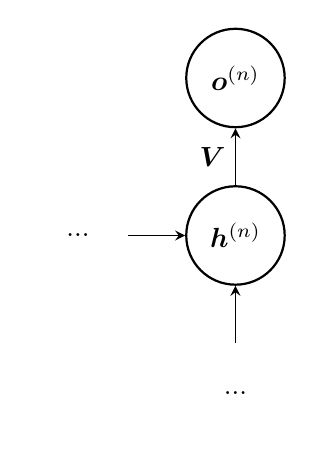
\begin{tikzpicture}[>=stealth, auto, node distance=2cm, semithick]
\tikzstyle{every state}=[draw=black, thick, fill=white, minimum size=1.25cm]

\node[state] (hn) {$\bm{h}^{(n)}$};
\node[state] (on) [above of=hn] {$\bm{o}^{(n)}$};
\node[state][draw=white] (ht) [left of=hn] {...};
\node[state][draw=white] (xt) [below of=hn] {...};

\path[->] (xt) edge node {} (hn);
\path[->] (ht) edge node {} (hn);
\path[->] (hn) edge node {$\bm{V}$} (on);
\end{tikzpicture}
\caption{Computational graph showing gradients for $\bm{h}^{(n)}$}
\label{fig:grad-hn}
\end{figure}

\begin{equation}
\label{eqn:backward-hn}
\begin{split}
	\frac{\partial L}{\partial \bm{h}^{(n)}}
		&= \frac{\partial L}{\partial \bm{o}^{(n)}} \frac{\partial \bm{o}^{(n)}}{\partial \bm{h}^{(n)}} \\
		&= (\hat{\bm{y}}^{(n)} - \bm{y}^{(n)}) \frac{\partial(\bm{c} + \bm{V}\bm{h}^{(n)})}{\partial \bm{h}^{(n)}} \\
		&= \bm{V}^T(\hat{\bm{y}}^{(n)} - \bm{y}^{(n)})
\end{split}
\end{equation}

Now, we can formulate the rest of the gradients recursively.

\begin{figure}[h!]
\centering
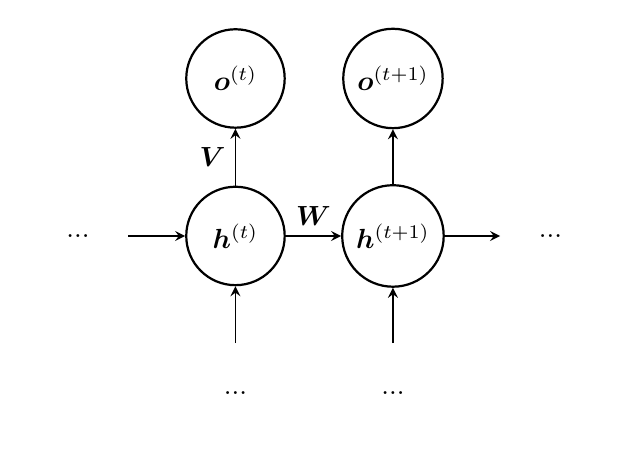
\begin{tikzpicture}[>=stealth, auto, node distance=2cm, semithick]
\tikzstyle{every state}=[draw=black, thick, fill=white, minimum size=1.25cm]

\node[state] (ht) {$\bm{h}^{(t)}$};
\node[state] (ot) [above of=ht] {$\bm{o}^{(t)}$};
\node[state] (ht+1) [right of=ht]{$\bm{h}^{(t+1)}$};
\node[state] (ot+1) [above of=ht+1] {$\bm{o}^{(t+1)}$};
\node[state][draw=white] (ht-1) [left of=ht] {...};
\node[state][draw=white] (xt) [below of=ht] {...};
\node[state][draw=white] (ht+2) [right of=ht+1] {...};
\node[state][draw=white] (xt+1) [below of=ht+1] {...};

\path[->] (xt) edge node {} (ht);
\path[->] (xt+1) edge node {} (ht+1);

\path[->] (ht-1) edge node {} (ht);
\path[->] (ht) edge node {$\bm{W}$} (ht+1);
\path[->] (ht+1) edge node {} (ht+2);

\path[->] (ht) edge node {$\bm{V}$} (ot);
\path[->] (ht+1) edge node {} (ot+1);
\end{tikzpicture}
\caption{Computational graph showing gradients for $\bm{h}^{(t)}$}
\label{fig:grad-ht}
\end{figure}

	$$ \frac{\partial L}{\partial \bm{h}^{(t)}}
		= \frac{\partial L}{\partial \bm{o}^{(t)}} \frac{\partial \bm{o}^{(t)}}{\partial \bm{h}^{(t)}}
		+ \frac{\partial L}{\partial \bm{h}^{(t+1)}} \frac{\partial \bm{h}^{(t+1)}}{\partial \bm{h}^{(t)}} $$

From the result in Equation \ref{eqn:backward-hn}, we have that
	$$ \frac{\partial L}{\partial \bm{o}^{(t)}} \frac{\partial \bm{o}^{(t)}}{\partial \bm{h}^{(t)}}
		 = \bm{V}^T(\hat{\bm{y}}^{(t)} - \bm{y}^{(t)}) $$

\begin{equation*}
\begin{split}
	\frac{\partial L}{\partial \bm{h}^{(t+1)}} \frac{\partial \bm{h}^{(t+1)}}{\partial \bm{h}^{(t)}}
		&= \frac{\partial L}{\partial \bm{h}^{(t+1)}} \frac{\partial \bm{h}^{(t+1)}}{\partial \bm{a}^{(t+1)}} \frac{\partial \bm{a}^{(t+1)}}{\partial \bm{h}^{(t)}} \\
		&= \frac{\partial L}{\partial \bm{h}^{(t+1)}} \frac{\partial( \text{tanh}(\bm{a}^{(t+1)}))}{\partial \bm{a}^{(t+1)}} \frac{\partial (\bm{b} + \bm{U}\bm{x}^{(t+1)} + \bm{W}\bm{h}^{(t)})}{\partial \bm{h}^{(t)}} \\
		&= \bm{W}^T \frac{\partial L}{\partial \bm{h}^{(t+1)}} \frac{\partial( \text{tanh}(\bm{a}^{(t+1)}))}{\partial \bm{a}^{(t+1)}} \\
		&= \bm{W}^T \text{diag}(1 - (\bm{h}^{(t+1)})^2) \frac{\partial L}{\partial \bm{h}^{(t+1)}}
\end{split}
\end{equation*}

Combining the above results, we obtain
\begin{equation}
\label{eqn:backward-ht}
\begin{split}
	\frac{\partial L}{\partial \bm{h}^{(t)}}
		&= \frac{\partial L}{\partial \bm{o}^{(t)}} \frac{\partial \bm{o}^{(t)}}{\partial \bm{h}^{(t)}} 
			+ \frac{\partial L}{\partial \bm{h}^{(t+1)}} \frac{\partial \bm{h}^{(t+1)}}{\partial \bm{h}^{(t)}} \\
		&= \bm{V}^T(\hat{\bm{y}}^{(t)} - \bm{y}^{(t)}) + \bm{W}^T \text{diag}(1 - (\bm{h}^{(t+1)})^2) \frac{\partial L}{\partial \bm{h}^{(t+1)}}
\end{split}
\end{equation}

It is next imperative to show that the Jacobian $J^{(t+1)} = \frac{\partial \bm{h}^{(t+1)}}{\partial \bm{a}^{(t+1)}} = \frac{\partial( \text{tanh}(\bm{a}^{(t+1)}))}{\partial \bm{a}^{(t+1)}} = \text{diag}(1 - (\bm{h}^{(t+1)})^2)$. \\

We begin with the knowledge that $\frac{d}{dx}\text{tanh}(x) = 1 - \text{tanh}^2(x)$.
	$$ J^{(t+1)}_{ij} = \frac{\partial \bm{h}^{(t+1)}_i}{\partial \bm{a}^{(t+1)}_j} $$
For $i \ne j$, $J^{(t)}_{ij} = 0$. \\
For $i = j$,
\begin{equation*}
\begin{split}
	J^{(t+1)}_{ii} = \frac{\partial \bm{h}^{(t+1)}_i}{\partial \bm{a}^{(t+1)}_i} 
		&= \frac{\partial( \text{tanh}(\bm{a}^{(t+1)})_i)}{\partial \bm{a}^{(t+1)}_i} \\
		&= 1 - \text{tanh}^2 (\bm{a}^{(t+1)})_i \\
		&= 1 - (\bm{h}^{(t+1)}_i)^2
\end{split}
\end{equation*}

	$$ \therefore J^{(t)} = \frac{\partial \bm{h}^{(t)}}{\partial \bm{a}^{(t)}} =
		\begin{pmatrix}
		1 - (\bm{h}_1^{(t)})^2 & 0 & ... & 0 \\ 
		0 & 1 - (\bm{h}_2^{(t)})^2 & ... & 0 \\ 
		... & ... & 1 - (\bm{h}_i^{(t)})^2 & ... \\ 
		0 & 0 & ... & 1 - (\bm{h}_n^{(t)})^2
		\end{pmatrix} 
		= \text{diag}(1 - (\bm{h}^{(t)})^2) $$
		
We can then use this result to obtain the gradients with respect to $\bm{b}, \bm{W}, \bm{U}$.
\begin{equation}
\label{eqn:backward-b}
\begin{split}
	\frac{\partial L}{\partial \bm{b}}
		&= \sum_{t=1}^{n} \frac{\partial L}{\partial \bm{h}^{(t)}} \frac{\partial \bm{h}^{(t)}}{\partial \bm{a}^{(t)}} \frac{\partial \bm{a}^{(t)}}{\partial \bm{b}} \\
		&= \sum_{t=1}^{n} \text{diag}(1 - (\bm{h}^{(t)})^2) \frac{\partial L}{\partial \bm{h}^{(t)}} \frac{\partial (\bm{b} + \bm{U}\bm{x}^{(t)} + \bm{W}\bm{h}^{(t-1)})}{\partial \bm{b}} \\
		&= \sum_{t=1}^{n} \text{diag}(1 - (\bm{h}^{(t)})^2) \frac{\partial L}{\partial \bm{h}^{(t)}}
\end{split}
\end{equation}

\begin{equation}
\label{eqn:backward-W}
\begin{split}
	\frac{\partial L}{\partial \bm{W}}
		&= \sum_{t=1}^{n} \frac{\partial L}{\partial \bm{h}^{(t)}} \frac{\partial \bm{h}^{(t)}}{\partial \bm{a}^{(t)}} \frac{\partial \bm{a}^{(t)}}{\partial \bm{W}} \\
		&= \sum_{t=1}^{n} \text{diag}(1 - (\bm{h}^{(t)})^2) \frac{\partial L}{\partial \bm{h}^{(t)}} \frac{\partial (\bm{b} + \bm{U}\bm{x}^{(t)} + \bm{W}\bm{h}^{(t-1)})}{\partial \bm{W}} \\
		&= \sum_{t=1}^{n} \text{diag}(1 - (\bm{h}^{(t)})^2) \frac{\partial L}{\partial \bm{h}^{(t)}} \bm{h}^{(t-1)^T}
\end{split}
\end{equation}

\begin{equation}
\label{eqn:backward-U}
\begin{split}
	\frac{\partial L}{\partial \bm{U}}
		&= \sum_{t=1}^{n} \frac{\partial L}{\partial \bm{h}^{(t)}} \frac{\partial \bm{h}^{(t)}}{\partial \bm{a}^{(t)}} \frac{\partial \bm{a}^{(t)}}{\partial \bm{U}} \\
		&= \sum_{t=1}^{n} \text{diag}(1 - (\bm{h}^{(t)})^2) \frac{\partial L}{\partial \bm{h}^{(t)}} \frac{\partial (\bm{b} + \bm{U}\bm{x}^{(t)} + \bm{W}\bm{h}^{(t-1)})}{\partial \bm{U}} \\
		&= \sum_{t=1}^{n} \text{diag}(1 - (\bm{h}^{(t)})^2) \frac{\partial L}{\partial \bm{h}^{(t)}} \bm{x}^{(t)^T}
\end{split}
\end{equation}

In summary,
\begin{equation}
\label{eqn:backward-all}
\begin{split}
	\frac{\partial L}{\partial \bm{U}}
		&= \sum_{t=1}^{n} \text{diag}(1 - (\bm{h}^{(t)})^2) \frac{\partial L}{\partial \bm{h}^{(t)}} \bm{x}^{(t)^T} \\
	\frac{\partial L}{\partial \bm{W}}
		&= \sum_{t=1}^{n} \text{diag}(1 - (\bm{h}^{(t)})^2) \frac{\partial L}{\partial \bm{h}^{(t)}} \bm{h}^{(t-1)^T} \\
	\frac{\partial L}{\partial \bm{b}}
		&= \sum_{t=1}^{n} \text{diag}(1 - (\bm{h}^{(t)})^2) \frac{\partial L}{\partial \bm{h}^{(t)}} \\
	\frac{\partial L}{\partial \bm{V}}
		&= \sum_{t=1}^{n} (\hat{\bm{y}}^{(t)} - \bm{y}^{(t)}) \; \bm{h}^{(t)^T} \\
	\frac{\partial L}{\partial \bm{c}}
		&= \sum_{t=1}^{n} (\hat{\bm{y}}^{(t)} - \bm{y}^{(t)})
\end{split}
\end{equation}

\subsubsection{Training}


\subsubsection{Evaluation}


\subsubsection{Finetuning}


\subsubsection{Summary}

\end{document}
